\section{System Architecture}\label{systemarch}

Antidote has a plug-in based architecture. So, a Castalia plugin was developed to support communication between Antidote Stack and Castalia Modules. As the Antidote is developed to work with real devices, modifications had to be made to the library to work in Castalia Simulator. The communication, encoders, agent and manager are some of the Antidote's modules modified.

\subsection{Castalia Plugin}

Antidote itself is portable and uses ANSI C language to create a standard and clean library. To provide a communication between Antidote and other systems, like Castalia, we must adapt and develop the necessary communication plug-ins.

The proposed plug-in allows Castalia and Antidote to talk with each other through Castalia plug-in module. Inside Castalia, we can call any function from Antidote Library and retrieve any information from it, but transmitting data from Castalia to Antidote Library is not a simple task. To solve this, we first use external variables to make the data exchange between Castalia and Castalia plug-in module. Then, to obtain the data from Castalia plug-in module, Antidote uses pointers to Castalia plug-in functions that we call \textit{callback functions}. That is why we need a plug-in to mediate the communication. 

There is a set of callback functions in Castalia plug-in module that are passed to Antidote during the initialization process of each agent. These callback functions are passed to communication module of Antidote as pointers to functions. This way, whenever the communication module needs to retrieve or send a message, it just triggers the correspondent callback function. 
%The task of these callback functions is to receive and send messages as also initialize and finalize a agent network.

Figure~\ref{fig:CastaliaPlugin} depicts how Antidote gets messages from Castalia. The arriving messages are copied to an external variable in Castalia Simulator Module - the external variable is visible to both Castalia Simulator and Castalia Plugin module. Since the communication module in Antidote owns pointers to Castalia Plug-ins functions, it can retrieve the messages using callback functions.

\begin{figure}[htbp]
\centerline{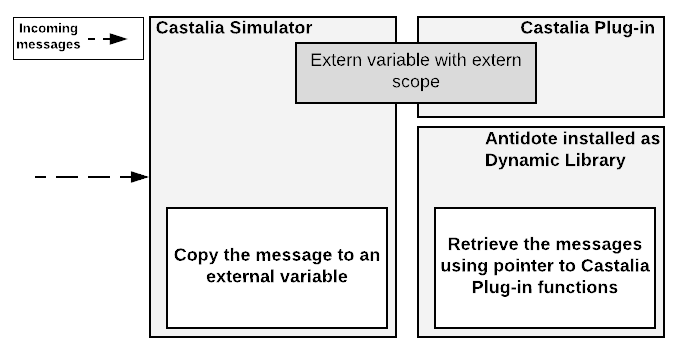
\includegraphics[scale=0.35]{figures/castaliaPlugin.png}}
\caption{How Antidote Library gets messages from Castalia Simulator.}
\label{fig:CastaliaPlugin}
\end{figure}

\subsection{Changes in communication module}

The Communication module is one of the most important modules in the Antidote Library. The start, the end, transmissions, machine state phases of all nodes are controlled by this module. In a real scenario, each device has its own communication module, running its own copy of the code. But in a single-machine simulation, it is a bit different. Only one communication module has to handle all nodes, since the Antidote Library is installed in the operating system as a dynamic library.

To ensure the proper operation of the Communication Module, the \textit{node id} is required in each function call, this way we know which node we are working with and apply the action for that node, without affecting other nodes. For example, if a node transits from unassociated state to associating machine state, without the proposed modification, this action would affect all nodes even those that should not change their machine states.

Figure~\ref{fig:communicationModuleCastalia} illustrates the system modification. In every function in the Communication module, we insert the \textit{node id} new parameter. This way the communication module always knows the corresponding node. 
%The arrows in Fig.~\ref{fig:communicationModuleCastalia} represents functions calls.

\begin{figure}[htbp]
\centerline{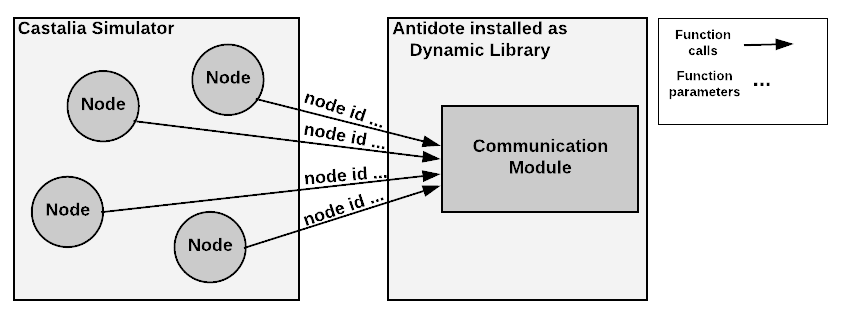
\includegraphics[scale=0.31]{figures/communicationModule.png}}
\caption{Communication module handling several nodes. Each arrow represents a function being called from the Communication Module.}
\label{fig:communicationModuleCastalia}
\end{figure}

\subsection{Other modifications}

Other modules like Agent, Manager and Encoders were modified to smooth operation of Antidote functions in Castalia. We can highlight the function created in the encoder module to convert absolute values (the measurements) into scaled non-negative values as recommended by \cite{b1}.
%Functions to finalize the Agents module were transferred to Manager module for the sake of simplicity and the \textit{node id} were add as a parameters of Agent and Manager functions.
%In Encoder module a function to interpret the data received was created.
It is useful to send absolute values like $-0.060$  which would require at least 4 bytes in X73-PHD floating point format. When converted, the number $-0.060$ becomes $388$, which requires just two bytes. The X73-PHD standard defines its own floating point types composed of a 32-bit word comprising a signed 8-bit integer exponent followed by a signed 24-bit integer mantissa.
%VINICIUS - acho melhor especificar pq falar só "many" fica muito genérico. R: feito.

Within the Manager, the equation to make the conversion from scaled to absolute values is given by expression\\$Y = M \times X + B$, where:
\begin{align*}
    Y &= \text{the converted absolute value}\\
    M &= \frac{(\text{upper absolute value} - \text{lower absolute value})}{(\text{upper scaled value} - \text{lower scaled value})}\\
    B &= \text{upper absolute value} - (M \times \text{upper scaled value})\\
    X &= \text{the scaled value}
\end{align*}

Within an Agent, the conversion from absolute values to scaled values is given by expression $X = \frac{(R - B)}{M}$, where: $R =$ actual measured value.

%\begin{align*}
%    R &= \text{actual measured value}
%\end{align*}

A thermometer that does readings from $-45^\circ$C  to $50^\circ$C with a resolution of $0.5^\circ$C has the following values: lower absolute value = $-45.0$, upper absolute value = $50.0$, lower scaled value = $0$, upper scaled value = $190$. Giving $M = 0.5$ and $B = -45.0$.

%\begin{align*}
%    \text{Lower absolute value} &= -45.0 \\
%    \text{Upper absolute value} &= 50.0 \\
%    \text{Lower scaled value} &= 0 \\
%    \text{Upper scaled value} &= 190
%\end{align*}

%Giving $M = \frac{(50.0 - (-45.0))}{(190 – 0)} = 0.5$ and $B = 50.0 - (0.5 \times 190) = -45.0$

The Castalia plug-in module and the modifications to Antidote Library were made exclusively for WBAN simulation in Castalia.

%VINICIUS - talvez uma conclusão dessa seção fosse inteiressante, R: Feito